\chapter{Kutatási eredmények}\label{ch:eredmenyek}

...

\section{A generatív mesterséges intelligencia megítélése}\label{genai-megiteles}

RQ1.

lustaságból használni jó, tudatlanságból használni veszélyes

junioroknak, betanulóknak egyre gyakrabban tiltják, mert ha az AI mondja meg a megoldást, nem rögzül igazán. a szenvedés (gondolkodás, megoldás megtalálása) rögzíti a tudást (a matematikához nem vezet királyi út) -- enélkül hasonló problémáknál nem fogjuk tudni használni ugyanezt a tudást\footnote{Az alapszakos egyetemi tanulmányaim legelején elsőként kezembe került jegyzet \parencite{bsz1} előszava idézte az anekdotát, ami szerint amikor I. Ptolemaiosz király megkérdezte Euklidészt, a kor nagy matematikusát, hogy nem lehetne-e a geometriát az Elemek \parencite{Elemek} áttanulmányozásánál könnyebben elsajátítani, Euklidész azt válaszolta: „A geometriához nem vezet királyi út. [...] Munka nélkül nincs kenyér, sem geometria.”}

kiváltja a juniorokat --> de akkor honnan lesznek később seniorok?

\section{A generatív mesterséges intelligencia felhasználása}\label{genai-felhasznalas}

RQ2 és RQ3 egyben, SDLC fázisonként

brainstorming postitek eloszlása

\begin{figure}
	\centering
	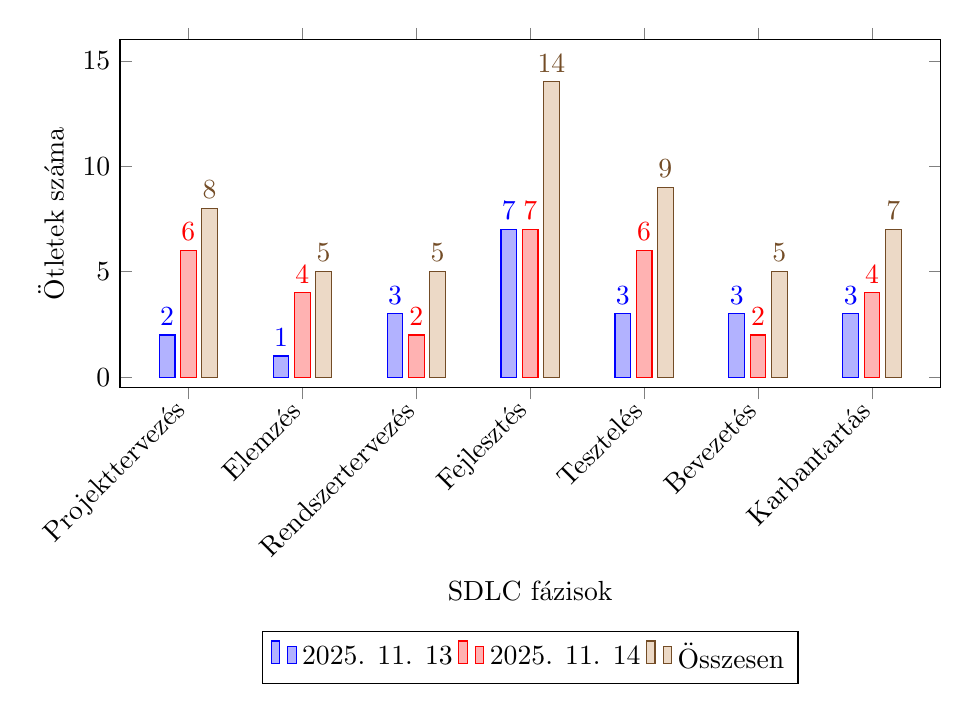
\begin{tikzpicture}
		\begin{axis}[
			xlabel={SDLC fázisok},
			ylabel={Ötletek száma},
			ybar,
			bar width=0.2cm,
			width=12cm,
			height=6cm,
			ymax=16,
			legend style={at={(0.5,-0.7)}, anchor=north, legend columns=3},
			xtick={1,2,3,4,5,6,7},
			xticklabels={Projekttervezés, Elemzés, Rendszertervezés, Fejlesztés, Tesztelés, Bevezetés, Karbantartás},
			x tick label style={rotate=45, anchor=east},
			ylabel near ticks,
			nodes near coords,
			]
			
			\addplot coordinates {(1,2) (2,1) (3,3) (4,7) (5,3) (6,3) (7,3)};
			\addlegendentry{2025. 11. 13}
			
			\addplot coordinates {(1,6) (2,4) (3,2) (4,7) (5,6) (6,2) (7,4)};
			\addlegendentry{2025. 11. 14}
			
			\addplot coordinates {(1,8) (2,5) (3,5) (4,14) (5,9) (6,5) (7,7)};
			\addlegendentry{Összesen}
		\end{axis}
	\end{tikzpicture}
	\caption{Az ötletek eloszlása SDLC fázisok szerint}
	\label{fig:sdlc_brainstorming}
\end{figure}

számos felhasználás már nemgeneratív MI-vel is volt, de generatívval kényelmesebb (még ha nem is feltétlenül jobb)
a sok pontosabb céleszköz vs. egy kevésbé pontos általános eszköz dilemma a pontosság és a hatékonyság között, lásd \parencite{mckinsey2025aipdlc}

A generatív mesterséges intelligencia potenciálisan hatékonyabbá teszi a szoftverfejlesztést, vagyis a fejlesztők bizonyos feladatokat rövidebb idő alatt tudnak elvégezni, mint korábban. Mivel így kevesebb időt kell bizonyos technikai részekkel eltölteniük, több idejük marad magasabb szintű tervezésre, munkatársakkal együtt gondolkodásra, új technológiák elsajátítására \cite{github_genai_devtime}.

A technológia felhasználásának fókuszában a kódolás áll \parencite{Gartner_AICodeAssistants_2025}, amit az ötletek eloszlása is alátámaszt (\ref{fig:sdlc_brainstorming}. ábra). Fontos azonban látni, hogy a szoftverfejlesztők a munkaidejük jóval kisebb részét töltik kódolással, mint azt akár ők, akár a menedzsereik gondolják \parencite{SoftwareCom_CodeTimeReport, today_was_a_good_day}. Éppen ezért a kódolási asszisztensek produktivitásnövelő hatása a teljes szoftverfejlesztési folyamatra vetítve nagyon korlátos. Olyan eszközökre van szükség, amelyek a generatív mesterséges intelligencia segítségével az SDLC valamennyi fázisát hatékonyabbá teszik \parencite{gartner_ai_sdlc}.

\subsection{Projekttervezés}

széles, de nem mély research, csak pointerek keresése, hogy merre érdemes indulni

ötletgyűjtés: mit lenne érdemes csinálni

aktuális helyzet/működés felmérése

adatok elemzése, pl. fontos-e egyáltalán a feature? (használják-e a rendelkezésre álló adatok alapján)

kockázatok elemzése

ötlet challenge-elése, pro-kontra

erőforrás, ETA becslés

tervdokumentum generálás


\subsection{Elemzés}

megvalósíthatóság elemzése

külső dokumentumok elemzése (azokból származó követelmények): adatok alapján követelmények meghatározása

követelmény megfogalmazás ellenőrzése, hiányzó követelmények keresése

\subsection{Rendszertervezés}

eszköz/technológia választás: lehetőségek keresése, megoldási lehetőségek összehasonlítása

prototípusok elkészítése: POC/MVP, infrastruktúra, egyszerű UI generálása

komplett rendszerterv legenerálása nagyon veszélyes: ki fogja azt tényleg olyan részletesen átnézni, mint amennyire ahhoz át kellett volna gondolni, hogy ő maga megcsinálja? túl nagy mennyiségű információ



\subsection{Fejlesztés}

kódgenerálás: nem kritikus, kevés mentális energiát igénylő dolgok (pl. boilerplate, UI)
komplex dolgokra hibás eredményt ad, a sok javítási iteráció fárasztóbb, mint megírni magát a kódot, végső soron nem spórolható meg a probléma végiggondolása \parencite{AI_pairprog}

refaktor: 

syntax error fix (pl. hosszú sql query), auto complete

kód megértése, elmagyarázása, dokumentálása (mit csinál)

scriptek (egyszerű, egyértelmű feladatok, olyan nyelven, amivel ritkán dolgozunk, tehát nem ismerjük, pl. awk, bash)

reguláris kifejezés (regular expression, regex) írás/értelmezés

fájlformátumok közti konvertálás

AI generált kód: fordítás+CI/CD sok hibát megtalálhat, de script nyelveknél még rizikósabb, hogy valami csak futtataáskor élesben derül ki

\subsection{Tesztelés}

unit test generálás -- gond: white box test, ha a kódból generálja, nem igazi független teszt

backward compatibility check

regressziós teszt output elemzés

integration test: AI agent elindítja a komponenseket, teszteli a kommunikációt

tesztadat generálás -- korlát: nem szisztematikus

AI generált kód reviewja: ember nem vonódik be, ha AI írta a kódot, nehezebb és unalmasabb átnézni, főleg ha sok kódot generál

vannak hibák, amiket nem követnénk el, de ha elénk tesznek egy kódot, amiben ott van, nem vesszük észre (nehezebb észrevenni, mint nem elrontani)

de az ember által írt kód AI általi reviewja, ellenőrzése jó felhasználás

\subsection{Bevezetés}

review

dependency analysis

deploy config generálás

utódokumentálás: ha van deploy dokumentálás, technical/user guide generálás

folyamat definiáltsága a kulcs: ha nem egy jól meghatározott folyamat, az AI se fogja tudni
ha jól megahtározott folyamat, akkor viszont már eleve automatizálható, nem kell igazán AI

agentic AI elvégezheti a telepítést, de ahhoz hozzáférés kell éles rendszerhez, ami nagyon veszélyes

példa: AI letörölt egy éles adatbázist, amit utána le is tagadott https://www.businessinsider.com/replit-ceo-apologizes-ai-coding-tool-delete-company-database-2025-7

\subsection{Karbantartás}

bottleneck analysis

find error cause

ticket preprocess (hiányzó adat kitöltése, hasonló hibák keresése, logok keresése)

LLM customer service, customer feedback kérés